% !TEX root=../report.tex

\section{Experiments}
\label{sec:experiment}


\subsection{DQN}
\label{sec:experiment:dqn}


\subsubsection{One Agents vs. One Adversary Results}
\label{sec:experiment:dqn:1vs1}


\begin{figure}[h]
  \centering
  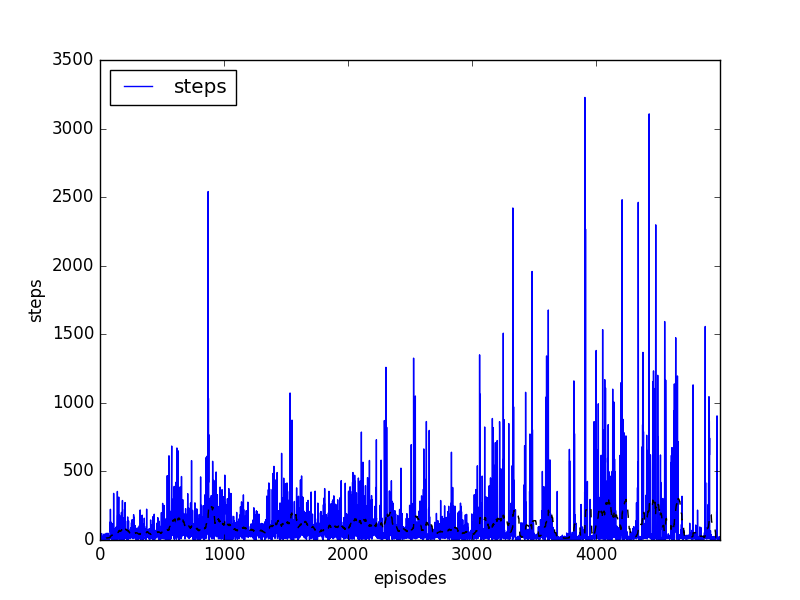
\includegraphics[trim=10 10 10 10,clip,width=\figscale\linewidth]
  {../results/dqn_1vs1/steps.png}
  \caption{Number of steps per episode over training episode for DQN.}
  \label{fig:dqn-1vs1}
\end{figure}
\FloatBarrier


\begin{figure}[h]
  \centering
  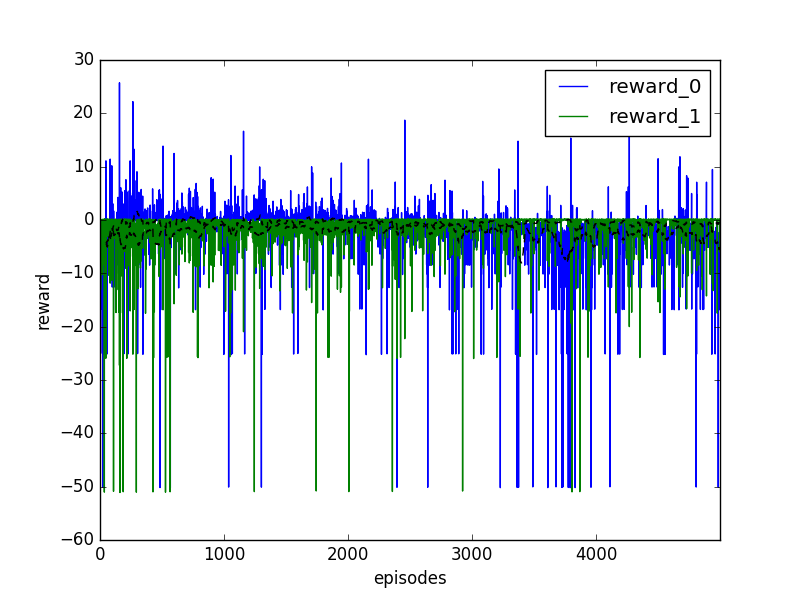
\includegraphics[trim=10 10 10 10,clip,width=\figscale\linewidth]
  {../results/dqn_1vs1/reward.png}
  \caption{Cumulative reward per episode over training episode for DQN.}
  \label{fig:dqn-1vs1}
\end{figure}
\FloatBarrier


\begin{figure}[h]
  \centering
  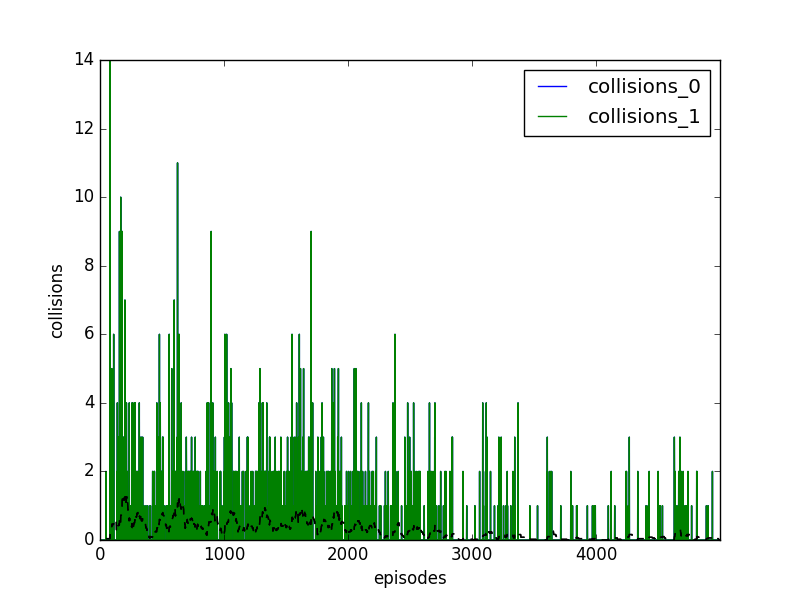
\includegraphics[trim=10 10 10 10,clip,width=\figscale\linewidth]
  {../results/dqn_1vs1/collisions.png}
  \caption{Number of collisions per episode over training episode for DQN.}
  \label{fig:dqn-1vs1}
\end{figure}
\FloatBarrier


\begin{figure}[h]
  \centering
  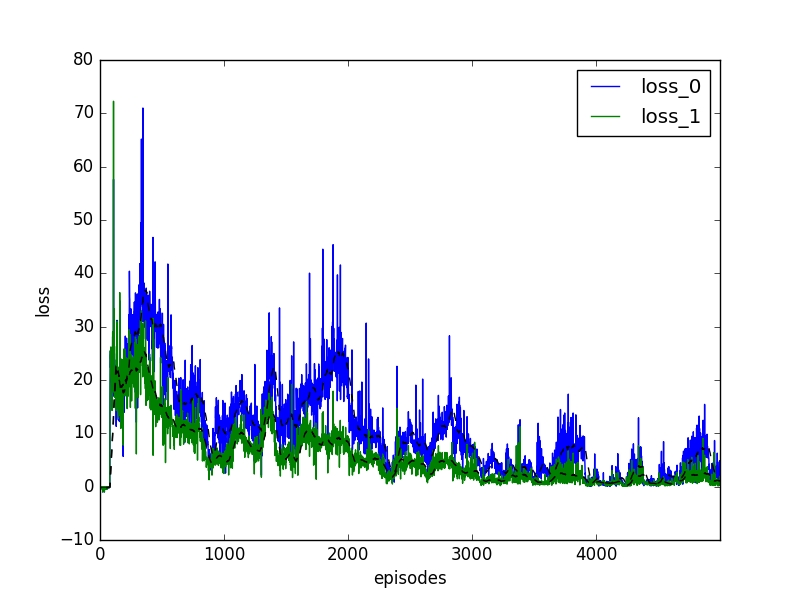
\includegraphics[trim=10 10 10 10,clip,width=\figscale\linewidth]
  {../results/dqn_1vs1/loss.png}
  \caption{Average loss per episode over training episode for DQN.}
  \label{fig:dqn-1vs1}
\end{figure}
\FloatBarrier


\subsubsection{Two Agents vs. One Adversary Results}
\label{sec:experiment:dqn:1vs2}


\begin{figure}[h]
  \centering
  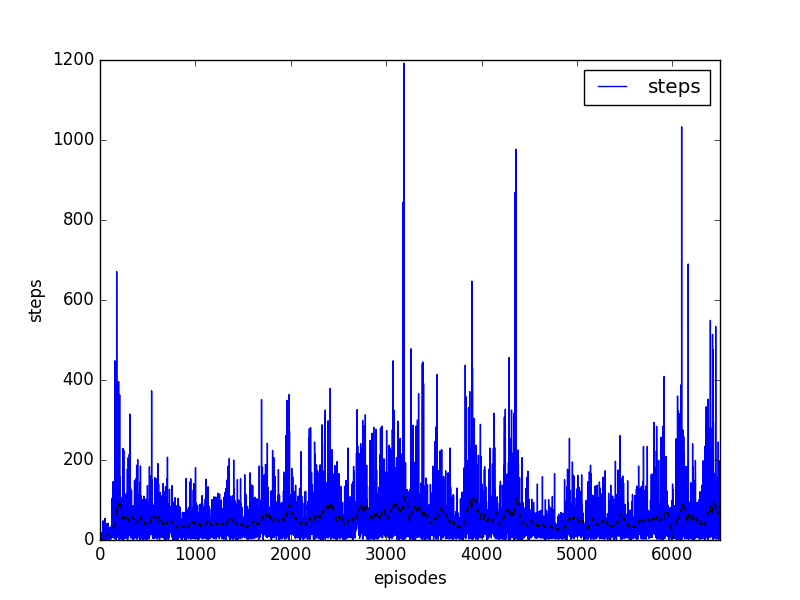
\includegraphics[trim=10 10 10 10,clip,width=\figscale\linewidth]
  {../results/dqn_1vs2/steps.png}
  \caption{Number of steps per episode over training episode for DQN.}
  \label{fig:dqn-1vs2}
\end{figure}
\FloatBarrier


\begin{figure}[h]
  \centering
  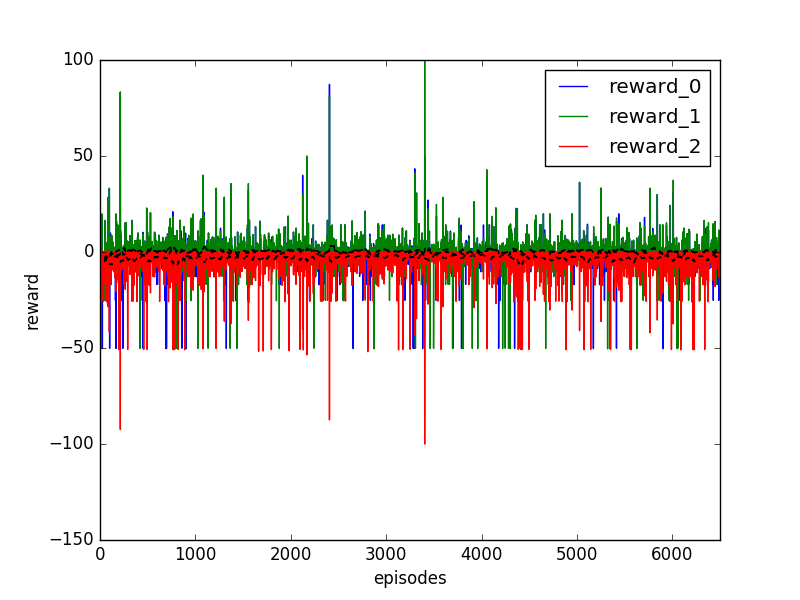
\includegraphics[trim=10 10 10 10,clip,width=\figscale\linewidth]
  {../results/dqn_1vs2/reward.png}
  \caption{Cumulative reward per episode over training episode for DQN.}
  \label{fig:dqn-1vs2}
\end{figure}
\FloatBarrier


\begin{figure}[h]
  \centering
  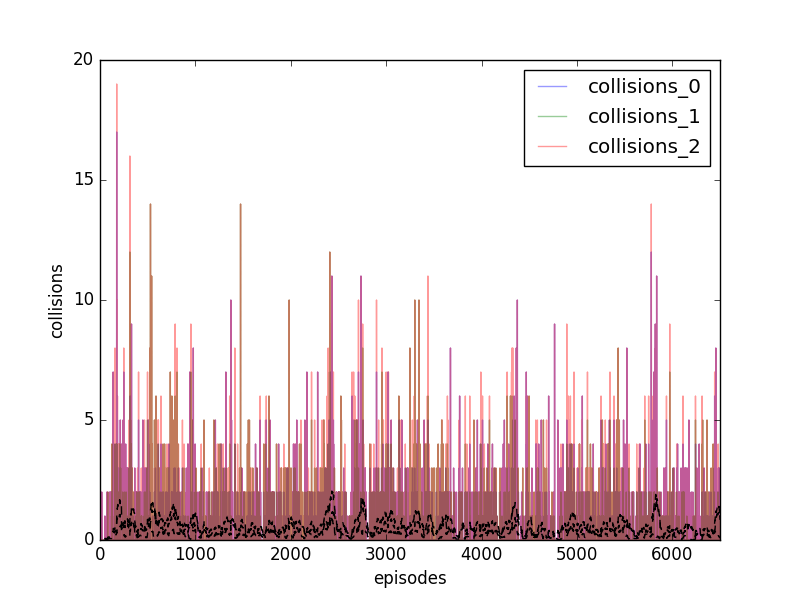
\includegraphics[trim=10 10 10 10,clip,width=\figscale\linewidth]
  {../results/dqn_1vs2/collisions.png}
  \caption{Number of collisions per episode over training episode for DQN.}
  \label{fig:dqn-1vs2}
\end{figure}
\FloatBarrier


\begin{figure}[h]
  \centering
  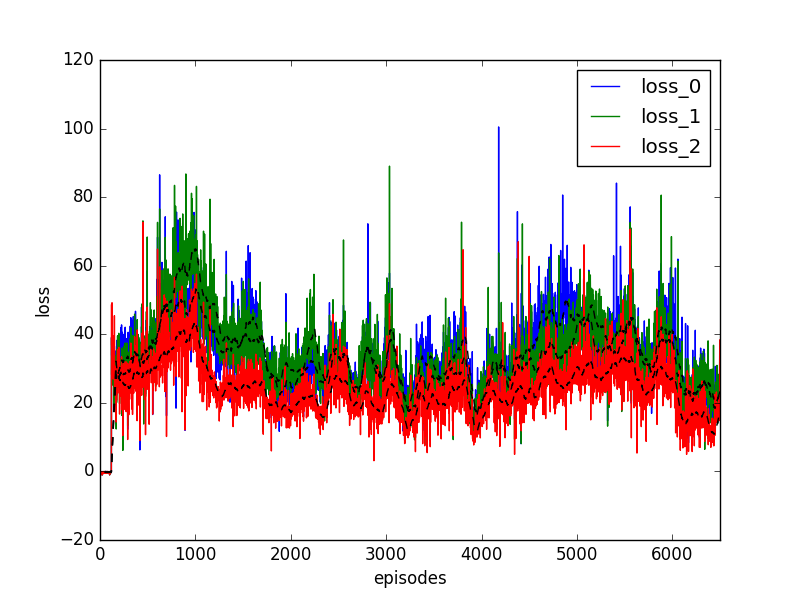
\includegraphics[trim=10 10 10 10,clip,width=\figscale\linewidth]
  {../results/dqn_1vs2/loss.png}
  \caption{Average loss per episode over training episode for DQN.}
  \label{fig:dqn-1vs2}
\end{figure}
\FloatBarrier


\subsubsection{One Agents vs. Two Adversary Results}
\label{sec:experiment:dqn:2vs1}


\begin{figure}[h]
  \centering
  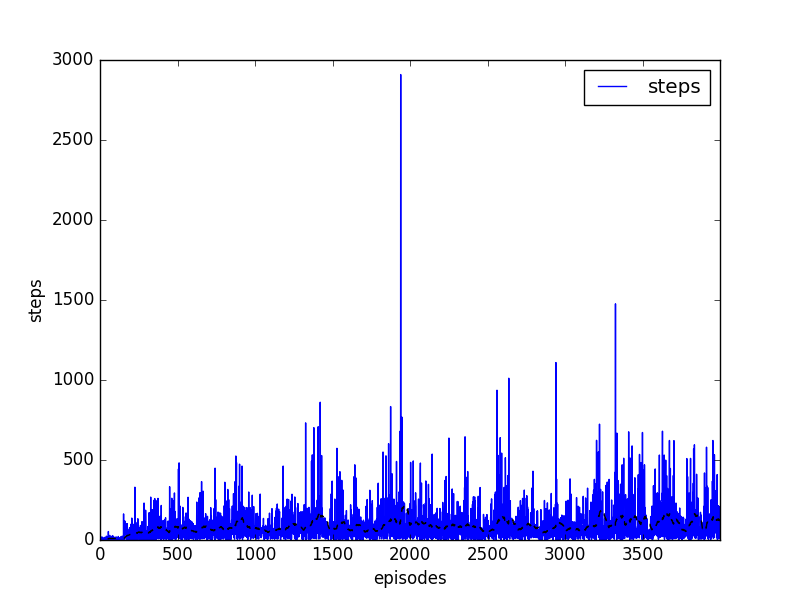
\includegraphics[trim=10 10 10 10,clip,width=\figscale\linewidth]
  {../results/dqn_2vs1/steps.png}
  \caption{Number of steps per episode over training episode for DQN.}
  \label{fig:dqn-2vs1}
\end{figure}
\FloatBarrier


\begin{figure}[h]
  \centering
  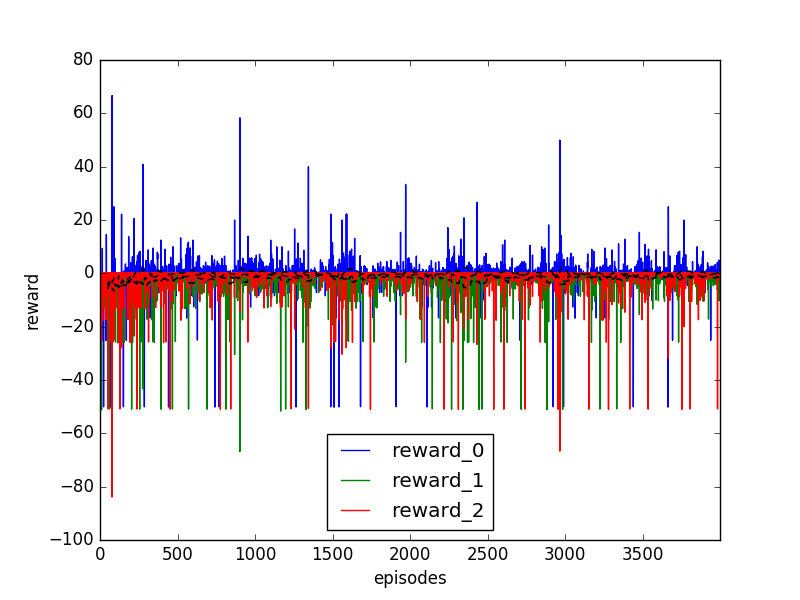
\includegraphics[trim=10 10 10 10,clip,width=\figscale\linewidth]
  {../results/dqn_2vs1/reward.png}
  \caption{Cumulative reward per episode over training episode for DQN.}
  \label{fig:dqn-2vs1}
\end{figure}
\FloatBarrier


\begin{figure}[h]
  \centering
  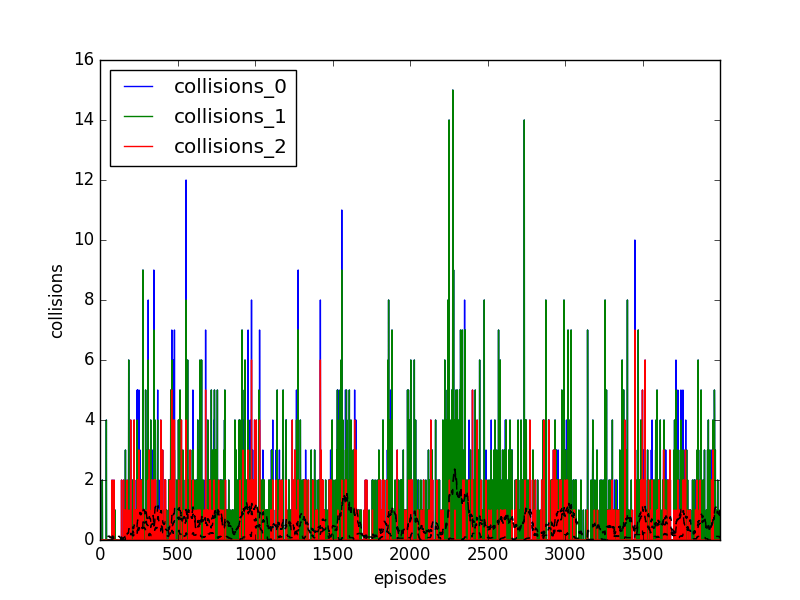
\includegraphics[trim=10 10 10 10,clip,width=\figscale\linewidth]
  {../results/dqn_2vs1/collisions.png}
  \caption{Number of collisions per episode over training episode for DQN.}
  \label{fig:dqn-2vs1}
\end{figure}
\FloatBarrier


\begin{figure}[h]
  \centering
  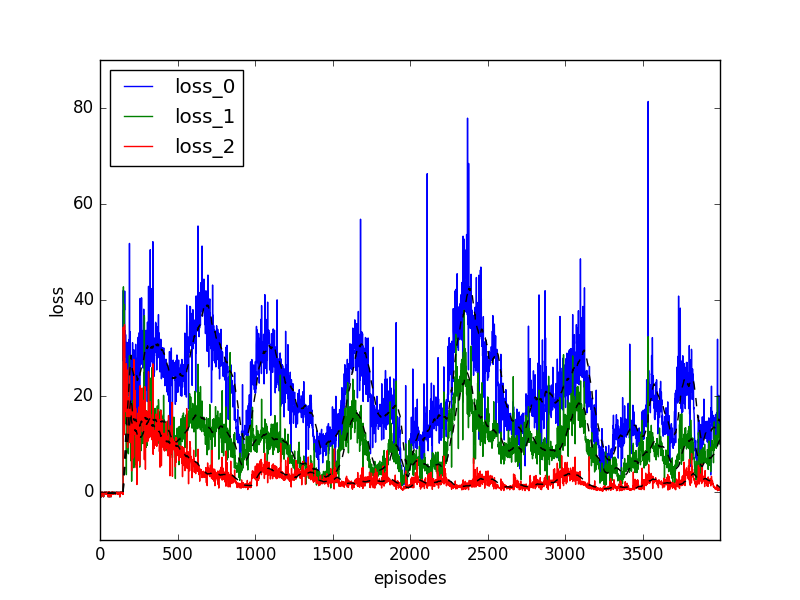
\includegraphics[trim=10 10 10 10,clip,width=\figscale\linewidth]
  {../results/dqn_2vs1/loss.png}
  \caption{Average loss per episode over training episode for DQN.}
  \label{fig:dqn-2vs1}
\end{figure}
\FloatBarrier


\subsection{DDPG}
\label{sec:experiment:ddpg}


\subsubsection{One Agents vs. One Adversary Results}
\label{sec:experiment:ddpg:1vs1}


\begin{figure}[h]
  \centering
  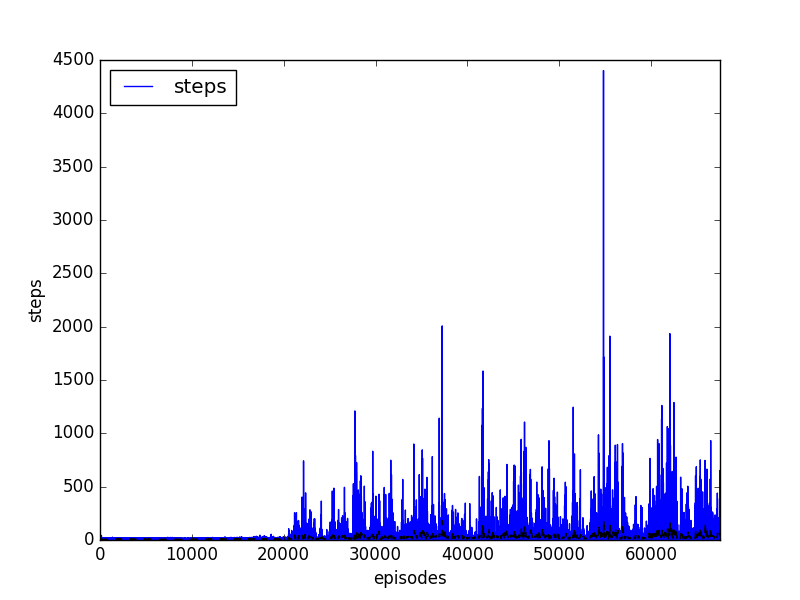
\includegraphics[trim=10 10 10 10,clip,width=\figscale\linewidth]
  {../results/ddpg_1vs1/steps.png}
  \caption{Number of steps per episode over training episode for DDPG.}
  \label{fig:ddpg-1vs1}
\end{figure}
\FloatBarrier


\begin{figure}[h]
  \centering
  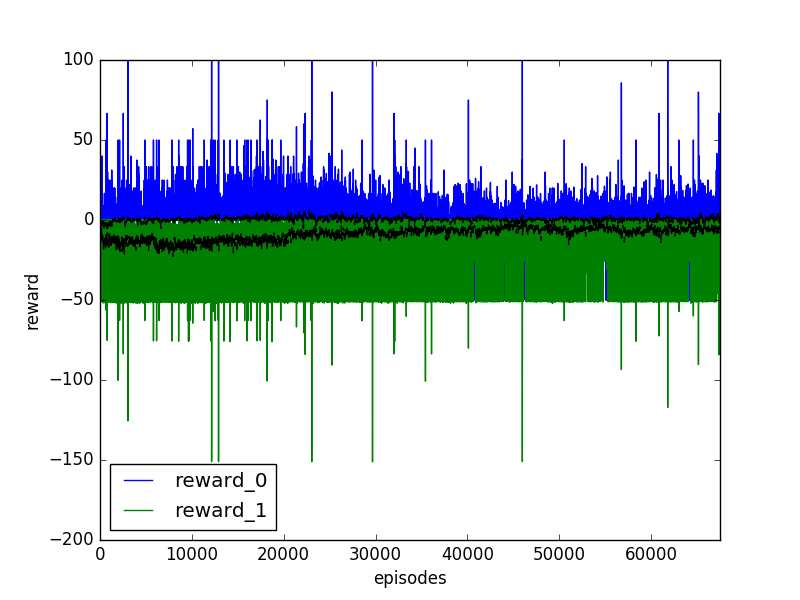
\includegraphics[trim=10 10 10 10,clip,width=\figscale\linewidth]
  {../results/ddpg_1vs1/reward.png}
  \caption{Cumulative reward per episode over training episode for DDPG.}
  \label{fig:ddpg-1vs1}
\end{figure}
\FloatBarrier


\begin{figure}[h]
  \centering
  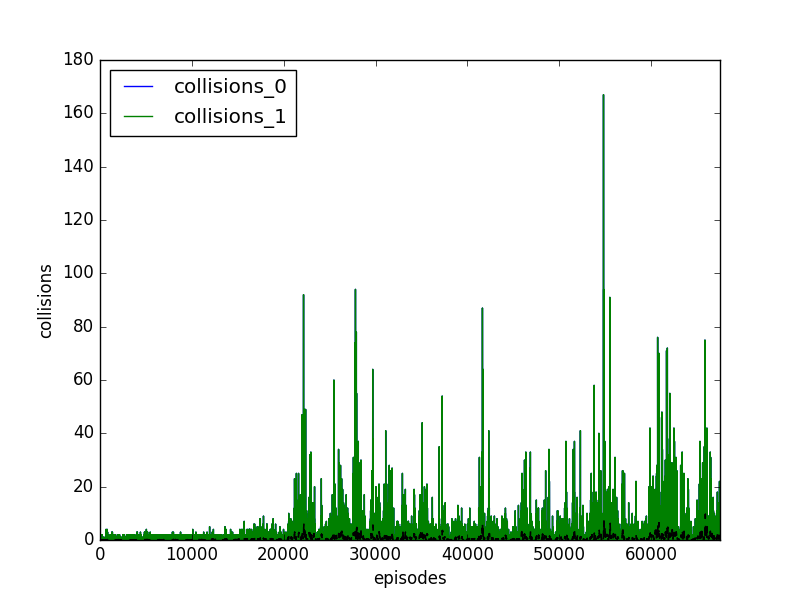
\includegraphics[trim=10 10 10 10,clip,width=\figscale\linewidth]
  {../results/ddpg_1vs1/collisions.png}
  \caption{Number of collisions per episode over training episode for DDPG.}
  \label{fig:ddpg-1vs1}
\end{figure}
\FloatBarrier


\begin{figure}[h]
  \centering
  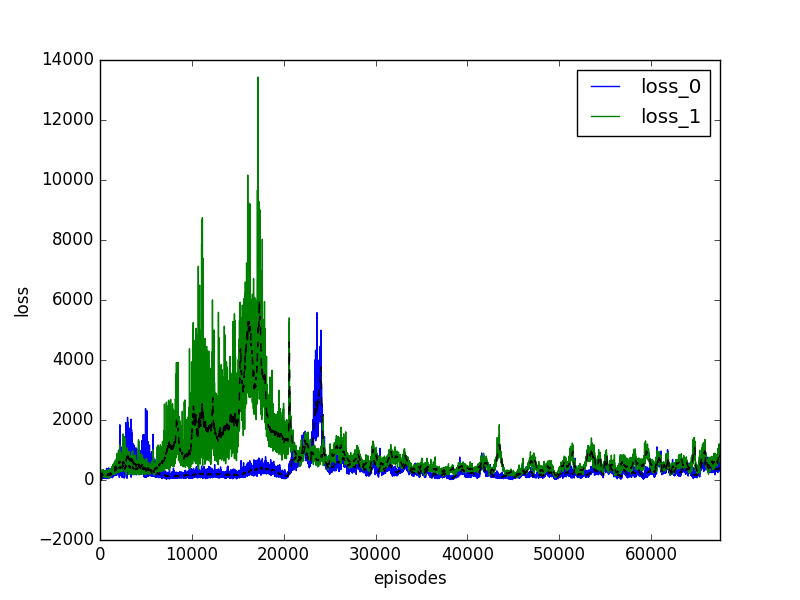
\includegraphics[trim=10 10 10 10,clip,width=\figscale\linewidth]
  {../results/ddpg_1vs1/loss.png}
  \caption{Average loss per episode over training episode for DDPG.}
  \label{fig:ddpg-1vs1}
\end{figure}
\FloatBarrier


\subsubsection{Two Agents vs. One Adversary Results}
\label{sec:experiment:ddpg:1vs2}


\begin{figure}[h]
  \centering
  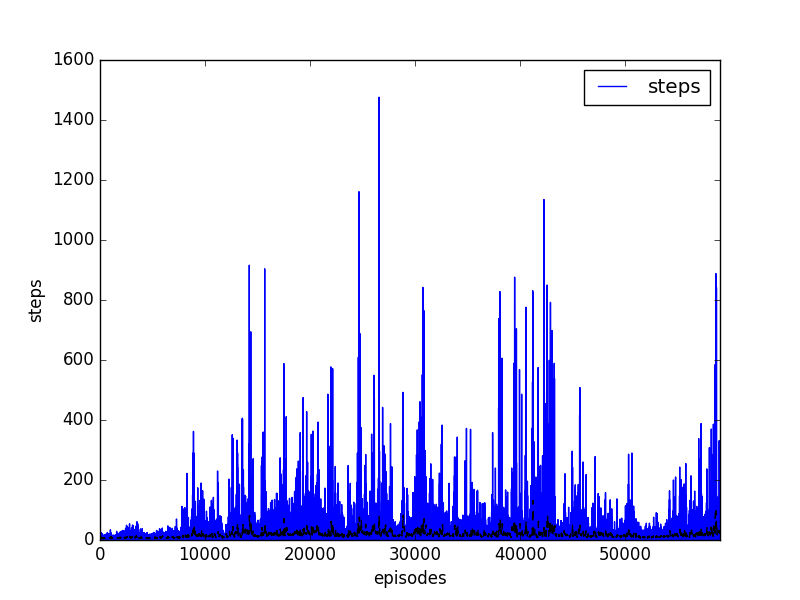
\includegraphics[trim=10 10 10 10,clip,width=\figscale\linewidth]
  {../results/ddpg_1vs2/steps.png}
  \caption{Number of steps per episode over training episode for DDPG.}
  \label{fig:ddpg-1vs2}
\end{figure}
\FloatBarrier


\begin{figure}[h]
  \centering
  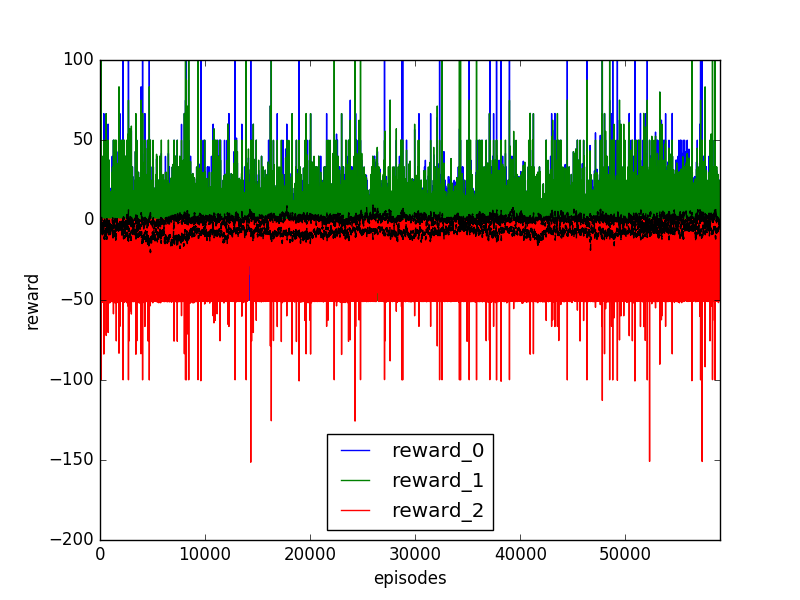
\includegraphics[trim=10 10 10 10,clip,width=\figscale\linewidth]
  {../results/ddpg_1vs2/reward.png}
  \caption{Cumulative reward per episode over training episode for DDPG.}
  \label{fig:ddpg-1vs2}
\end{figure}
\FloatBarrier


\begin{figure}[h]
  \centering
  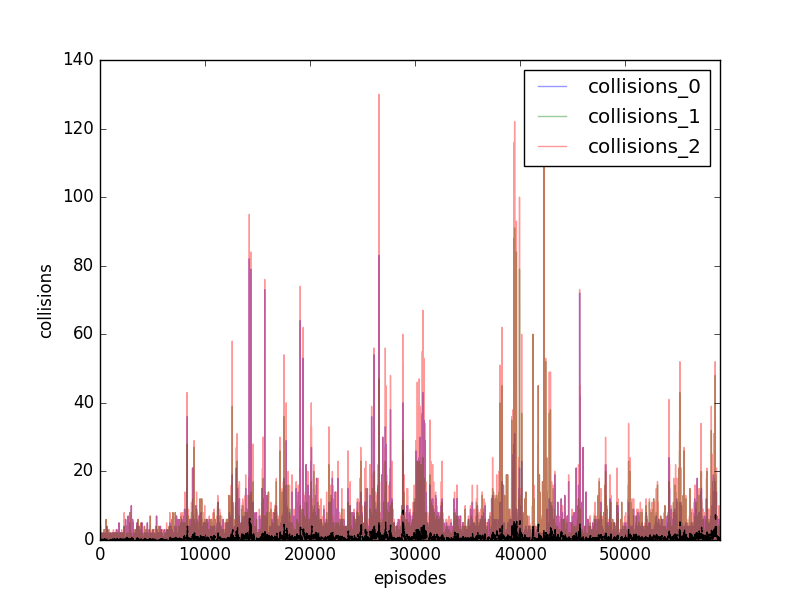
\includegraphics[trim=10 10 10 10,clip,width=\figscale\linewidth]
  {../results/ddpg_1vs2/collisions.png}
  \caption{Number of collisions per episode over training episode for DDPG.}
  \label{fig:ddpg-1vs2}
\end{figure}
\FloatBarrier


\begin{figure}[h]
  \centering
  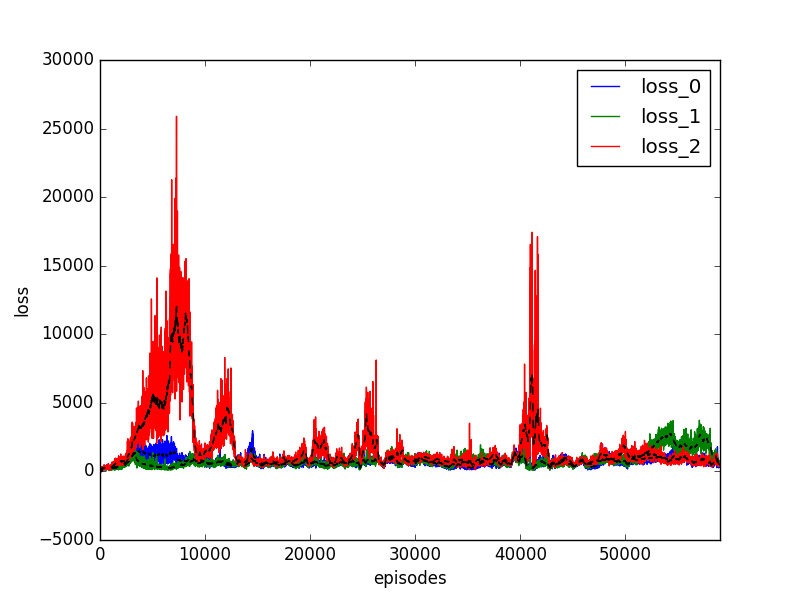
\includegraphics[trim=10 10 10 10,clip,width=\figscale\linewidth]
  {../results/ddpg_1vs2/loss.png}
  \caption{Average loss per episode over training episode for DDPG.}
  \label{fig:ddpg-1vs2}
\end{figure}
\FloatBarrier


\subsubsection{One Agents vs. Two Adversary Results}
\label{sec:experiment:ddpg:2vs1}


\begin{figure}[h]
  \centering
  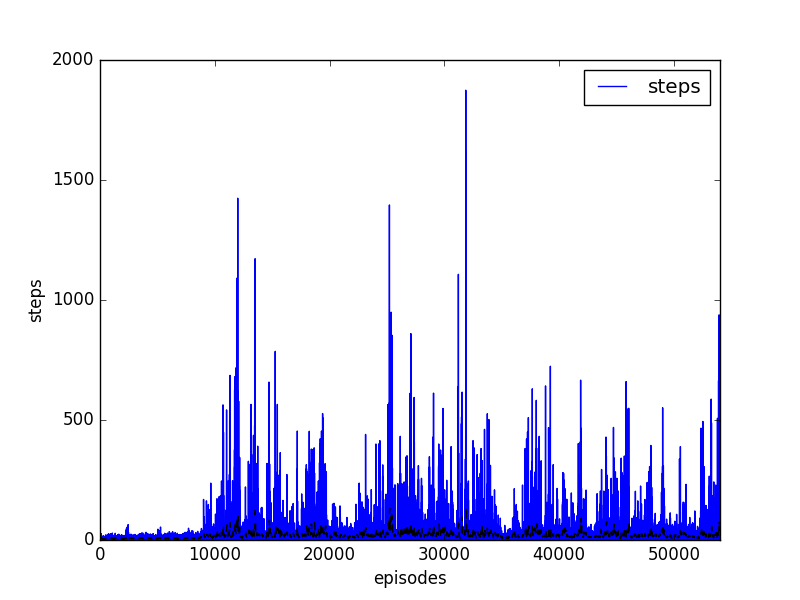
\includegraphics[trim=10 10 10 10,clip,width=\figscale\linewidth]
  {../results/ddpg_2vs1/steps.png}
  \caption{Number of steps per episode over training episode for DDPG.}
  \label{fig:ddpg-2vs1}
\end{figure}
\FloatBarrier


\begin{figure}[h]
  \centering
  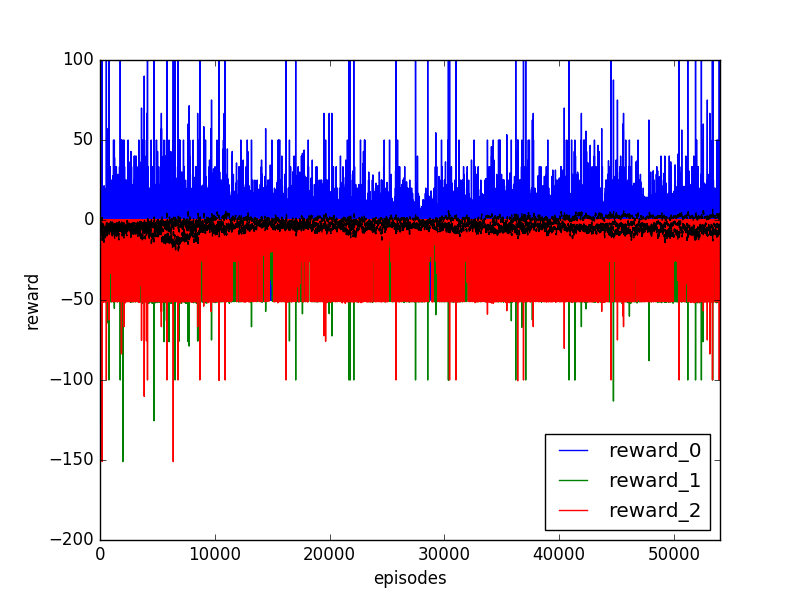
\includegraphics[trim=10 10 10 10,clip,width=\figscale\linewidth]
  {../results/ddpg_2vs1/reward.png}
  \caption{Cumulative reward per episode over training episode for DDPG.}
  \label{fig:ddpg-2vs1}
\end{figure}
\FloatBarrier


\begin{figure}[h]
  \centering
  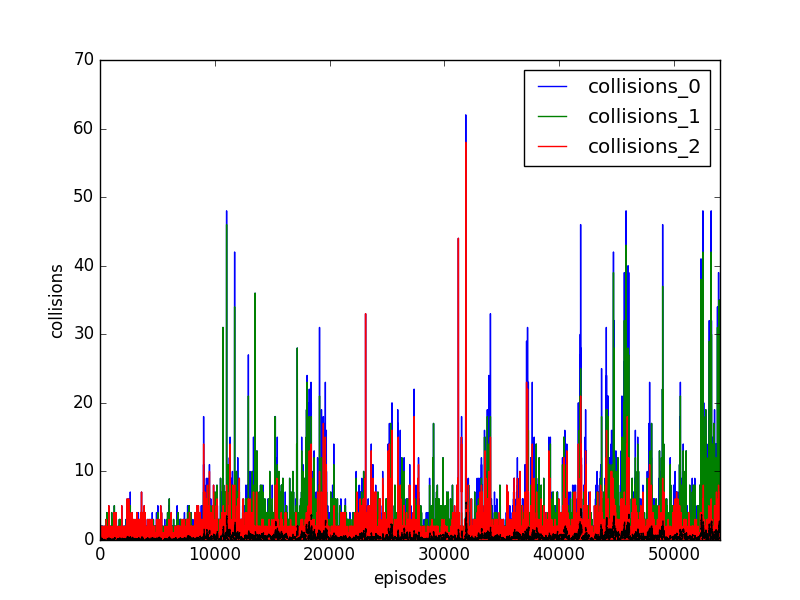
\includegraphics[trim=10 10 10 10,clip,width=\figscale\linewidth]
  {../results/ddpg_2vs1/collisions.png}
  \caption{Number of collisions per episode over training episode for DDPG.}
  \label{fig:ddpg-2vs1}
\end{figure}
\FloatBarrier


\begin{figure}[h]
  \centering
  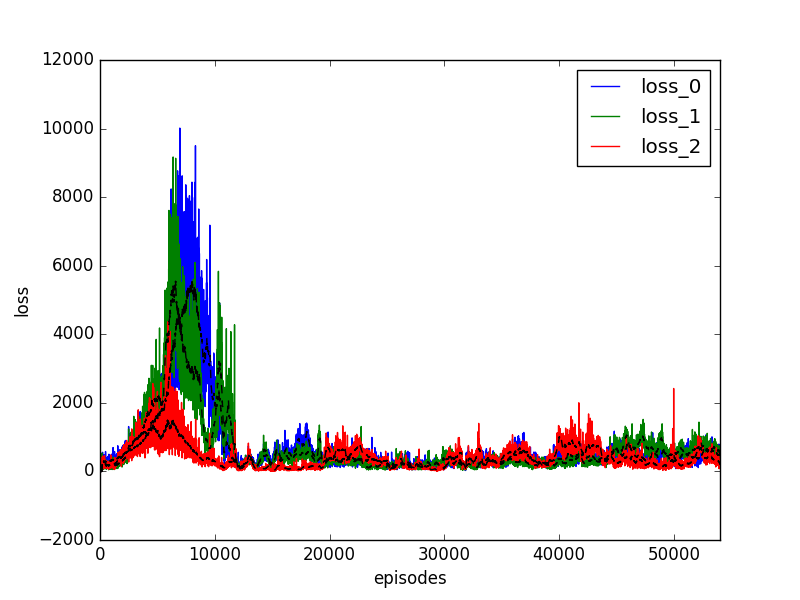
\includegraphics[trim=10 10 10 10,clip,width=\figscale\linewidth]
  {../results/ddpg_2vs1/loss.png}
  \caption{Average loss per episode over training episode for DDPG.}
  \label{fig:ddpg-2vs1}
\end{figure}
\FloatBarrier


\subsection{MADDPG}
\label{sec:experiment:maddpg}


\subsubsection{One Agents vs. One Adversary Results}
\label{sec:experiment:maddpg:1vs1}


\begin{figure}[h]
  \centering
  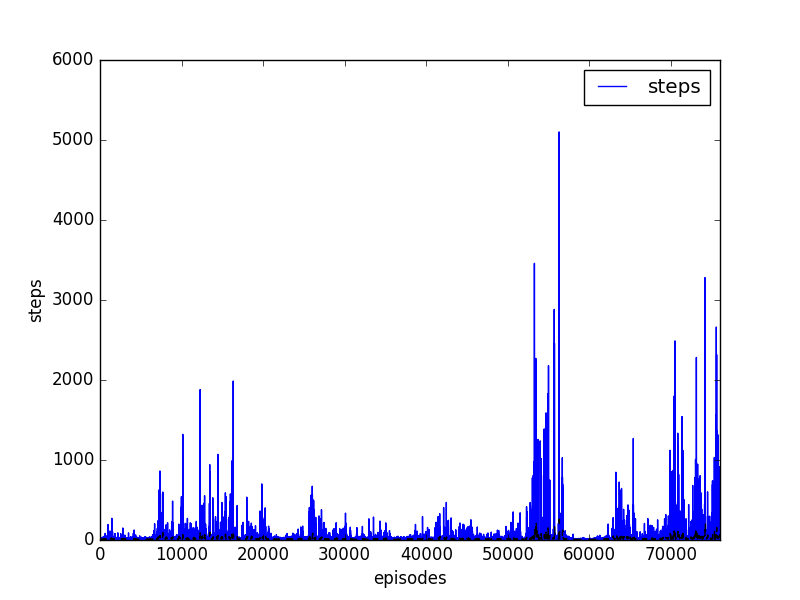
\includegraphics[trim=10 10 10 10,clip,width=\figscale\linewidth]
  {../results/maddpg_1vs1/steps.png}
  \caption{Number of steps per episode over training episode for MADDPG.}
  \label{fig:maddpg-1vs1}
\end{figure}
\FloatBarrier


\begin{figure}[h]
  \centering
  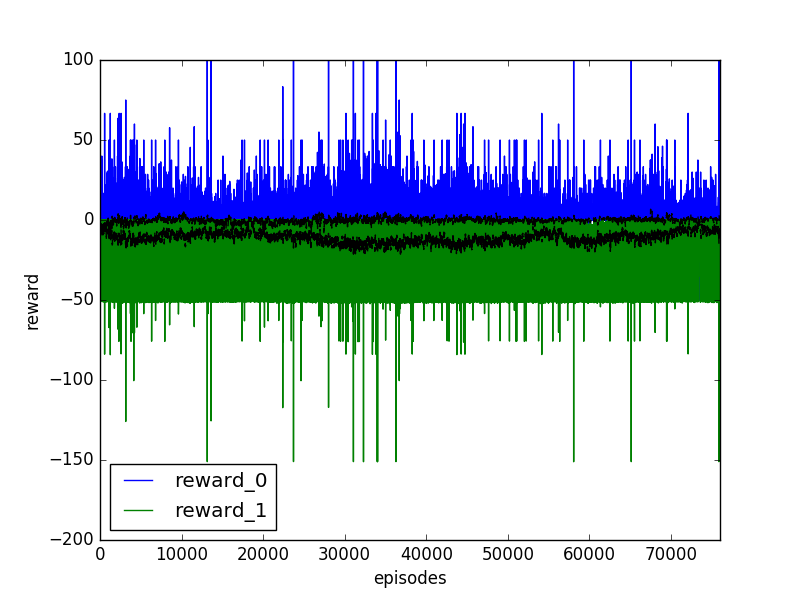
\includegraphics[trim=10 10 10 10,clip,width=\figscale\linewidth]
  {../results/maddpg_1vs1/reward.png}
  \caption{Cumulative reward per episode over training episode for MADDPG.}
  \label{fig:maddpg-1vs1}
\end{figure}
\FloatBarrier


\begin{figure}[h]
  \centering
  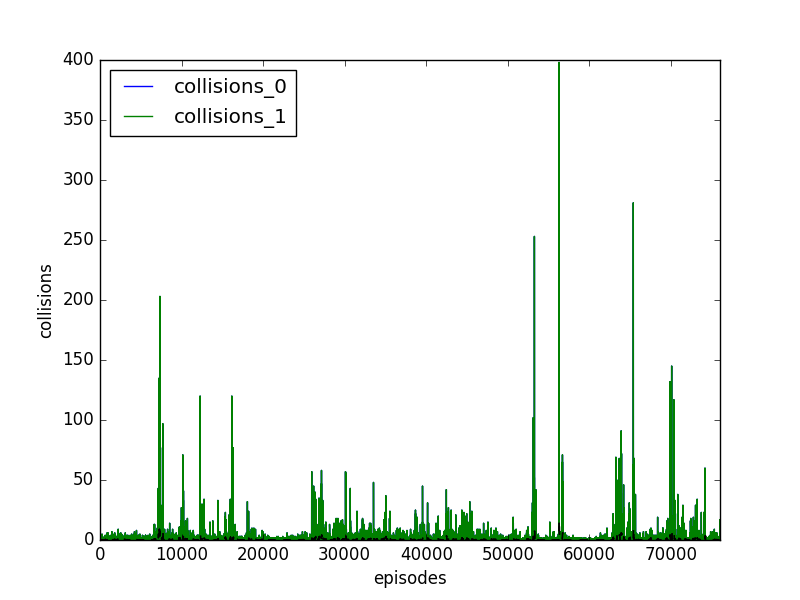
\includegraphics[trim=10 10 10 10,clip,width=\figscale\linewidth]
  {../results/maddpg_1vs1/collisions.png}
  \caption{Number of collisions per episode over training episode for MADDPG.}
  \label{fig:maddpg-1vs1}
\end{figure}
\FloatBarrier


\begin{figure}[h]
  \centering
  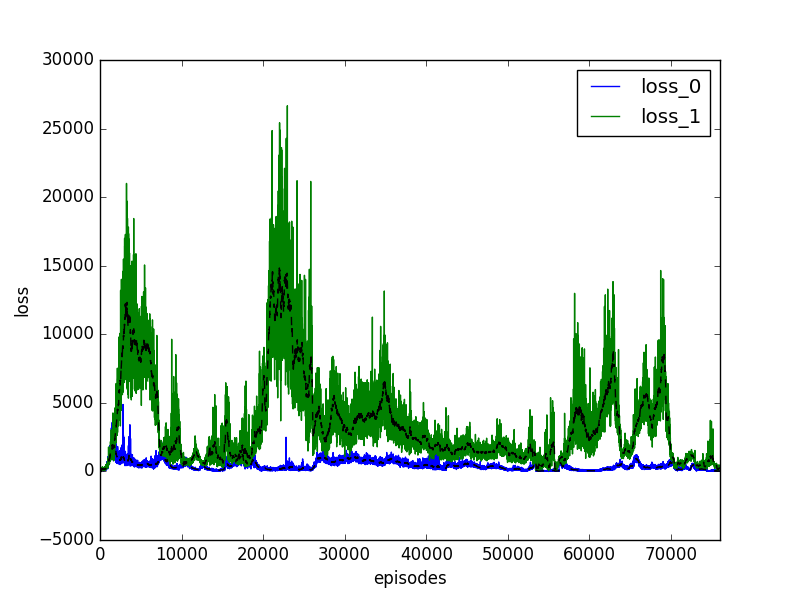
\includegraphics[trim=10 10 10 10,clip,width=\figscale\linewidth]
  {../results/maddpg_1vs1/loss.png}
  \caption{Average loss per episode over training episode for MADDPG.}
  \label{fig:maddpg-1vs1}
\end{figure}
\FloatBarrier


\subsubsection{Two Agents vs. One Adversary Results}
\label{sec:experiment:maddpg:1vs2}


\begin{figure}[h]
  \centering
  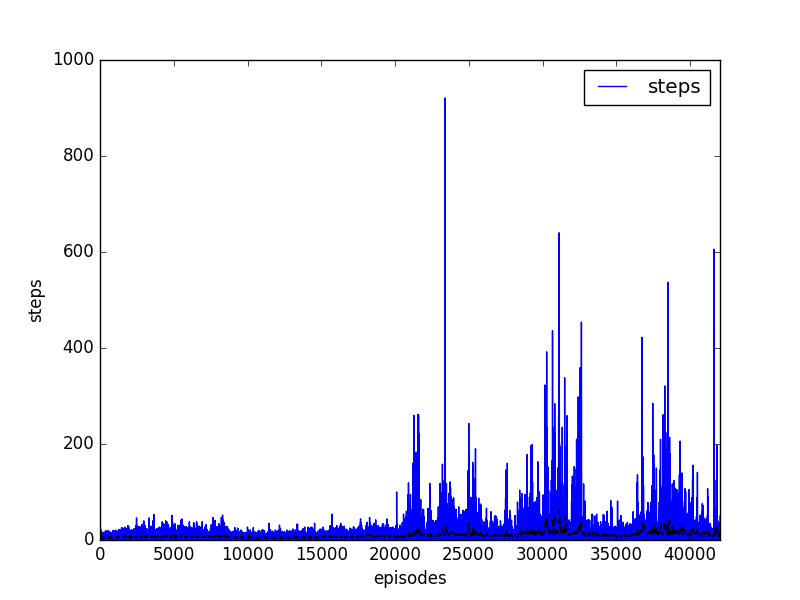
\includegraphics[trim=10 10 10 10,clip,width=\figscale\linewidth]
  {../results/maddpg_1vs2/steps.png}
  \caption{Number of steps per episode over training episode for MADDPG.}
  \label{fig:maddpg-1vs2}
\end{figure}
\FloatBarrier


\begin{figure}[h]
  \centering
  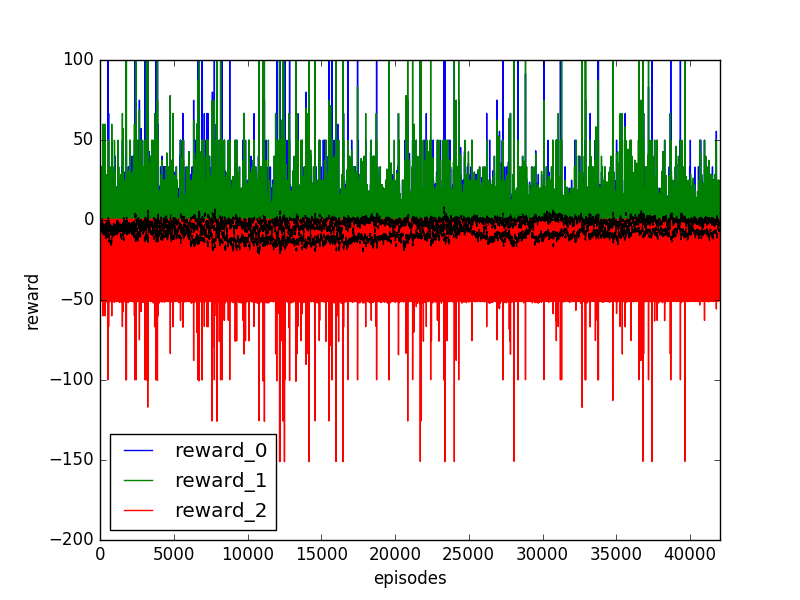
\includegraphics[trim=10 10 10 10,clip,width=\figscale\linewidth]
  {../results/maddpg_1vs2/reward.png}
  \caption{Cumulative reward per episode over training episode for MADDPG.}
  \label{fig:maddpg-1vs2}
\end{figure}
\FloatBarrier


\begin{figure}[h]
  \centering
  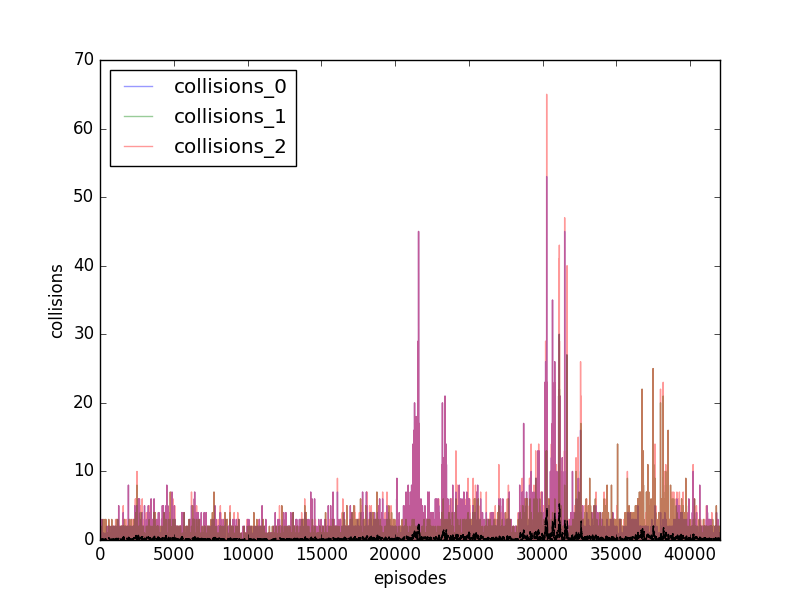
\includegraphics[trim=10 10 10 10,clip,width=\figscale\linewidth]
  {../results/maddpg_1vs2/collisions.png}
  \caption{Number of collisions per episode over training episode for MADDPG.}
  \label{fig:maddpg-1vs2}
\end{figure}
\FloatBarrier


\begin{figure}[h]
  \centering
  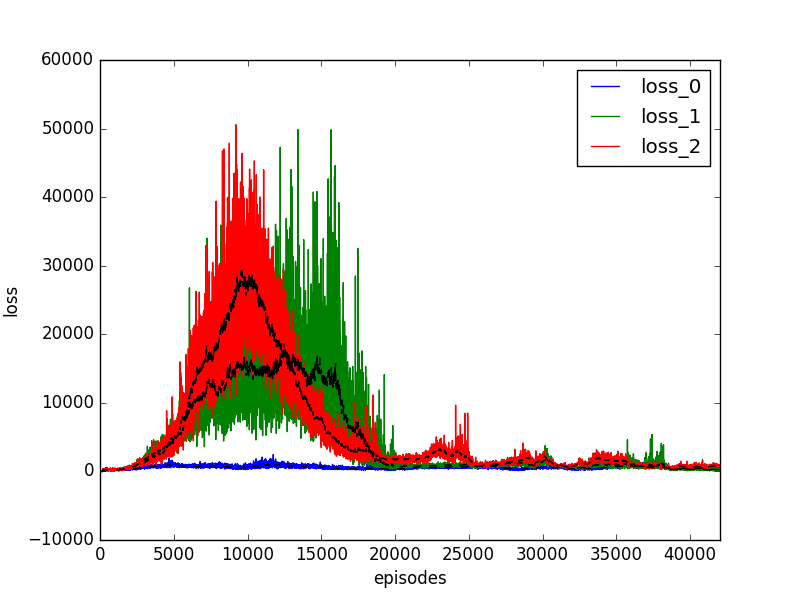
\includegraphics[trim=10 10 10 10,clip,width=\figscale\linewidth]
  {../results/maddpg_1vs2/loss.png}
  \caption{Average loss per episode over training episode for MADDPG.}
  \label{fig:maddpg-1vs2}
\end{figure}
\FloatBarrier


\subsubsection{One Agents vs. Two Adversary Results}
\label{sec:experiment:maddpg:2vs1}


\begin{figure}[h]
  \centering
  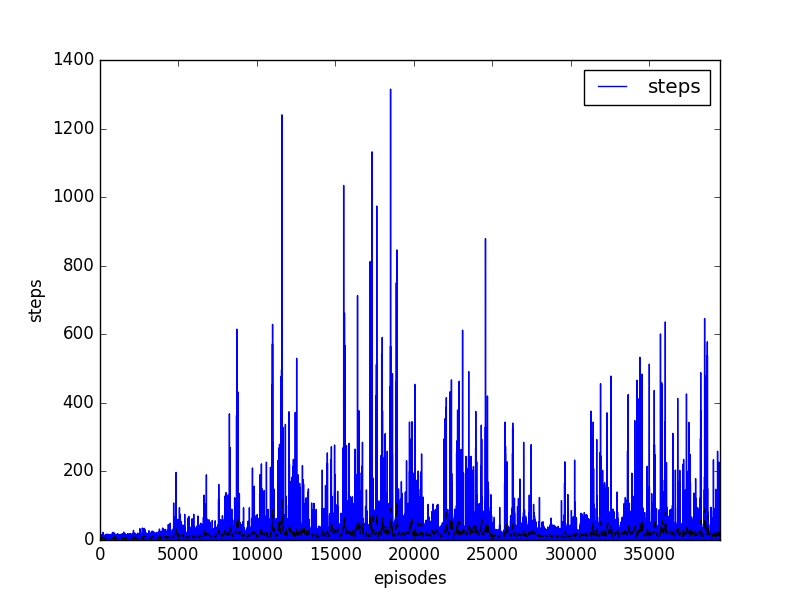
\includegraphics[trim=10 10 10 10,clip,width=\figscale\linewidth]
  {../results/maddpg_2vs1/steps.png}
  \caption{Number of steps per episode over training episode for MADDPG.}
  \label{fig:maddpg-2vs1}
\end{figure}
\FloatBarrier


\begin{figure}[h]
  \centering
  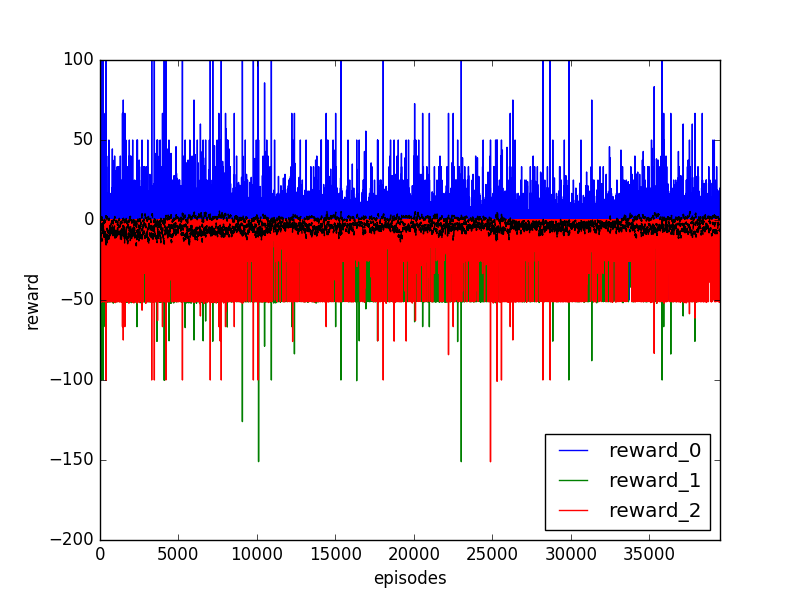
\includegraphics[trim=10 10 10 10,clip,width=\figscale\linewidth]
  {../results/maddpg_2vs1/reward.png}
  \caption{Cumulative reward per episode over training episode for MADDPG.}
  \label{fig:maddpg-2vs1}
\end{figure}
\FloatBarrier


\begin{figure}[h]
  \centering
  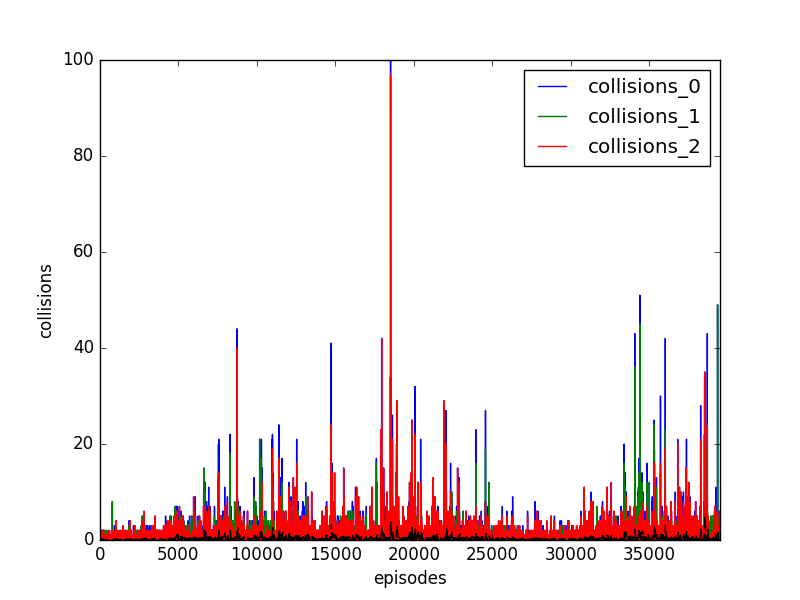
\includegraphics[trim=10 10 10 10,clip,width=\figscale\linewidth]
  {../results/maddpg_2vs1/collisions.png}
  \caption{Number of collisions per episode over training episode for MADDPG.}
  \label{fig:maddpg-2vs1}
\end{figure}
\FloatBarrier


\begin{figure}[h]
  \centering
  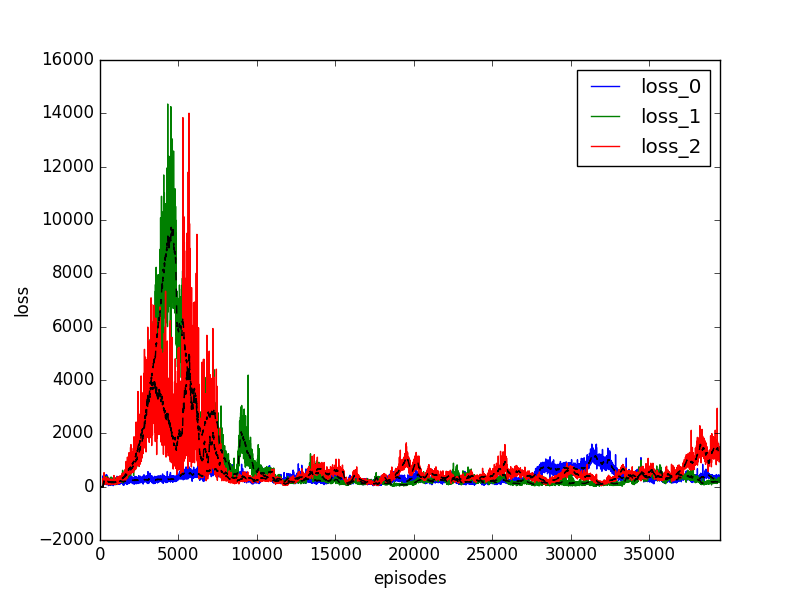
\includegraphics[trim=10 10 10 10,clip,width=\figscale\linewidth]
  {../results/maddpg_2vs1/loss.png}
  \caption{Average loss per episode over training episode for MADDPG.}
  \label{fig:maddpg-2vs1}
\end{figure}
\FloatBarrier

